% Copyright (c) 2015 Daniele Masini - d.masini.it@gmail.com

\chapter{Quadrilateri}\label{chap:quadrilateri}

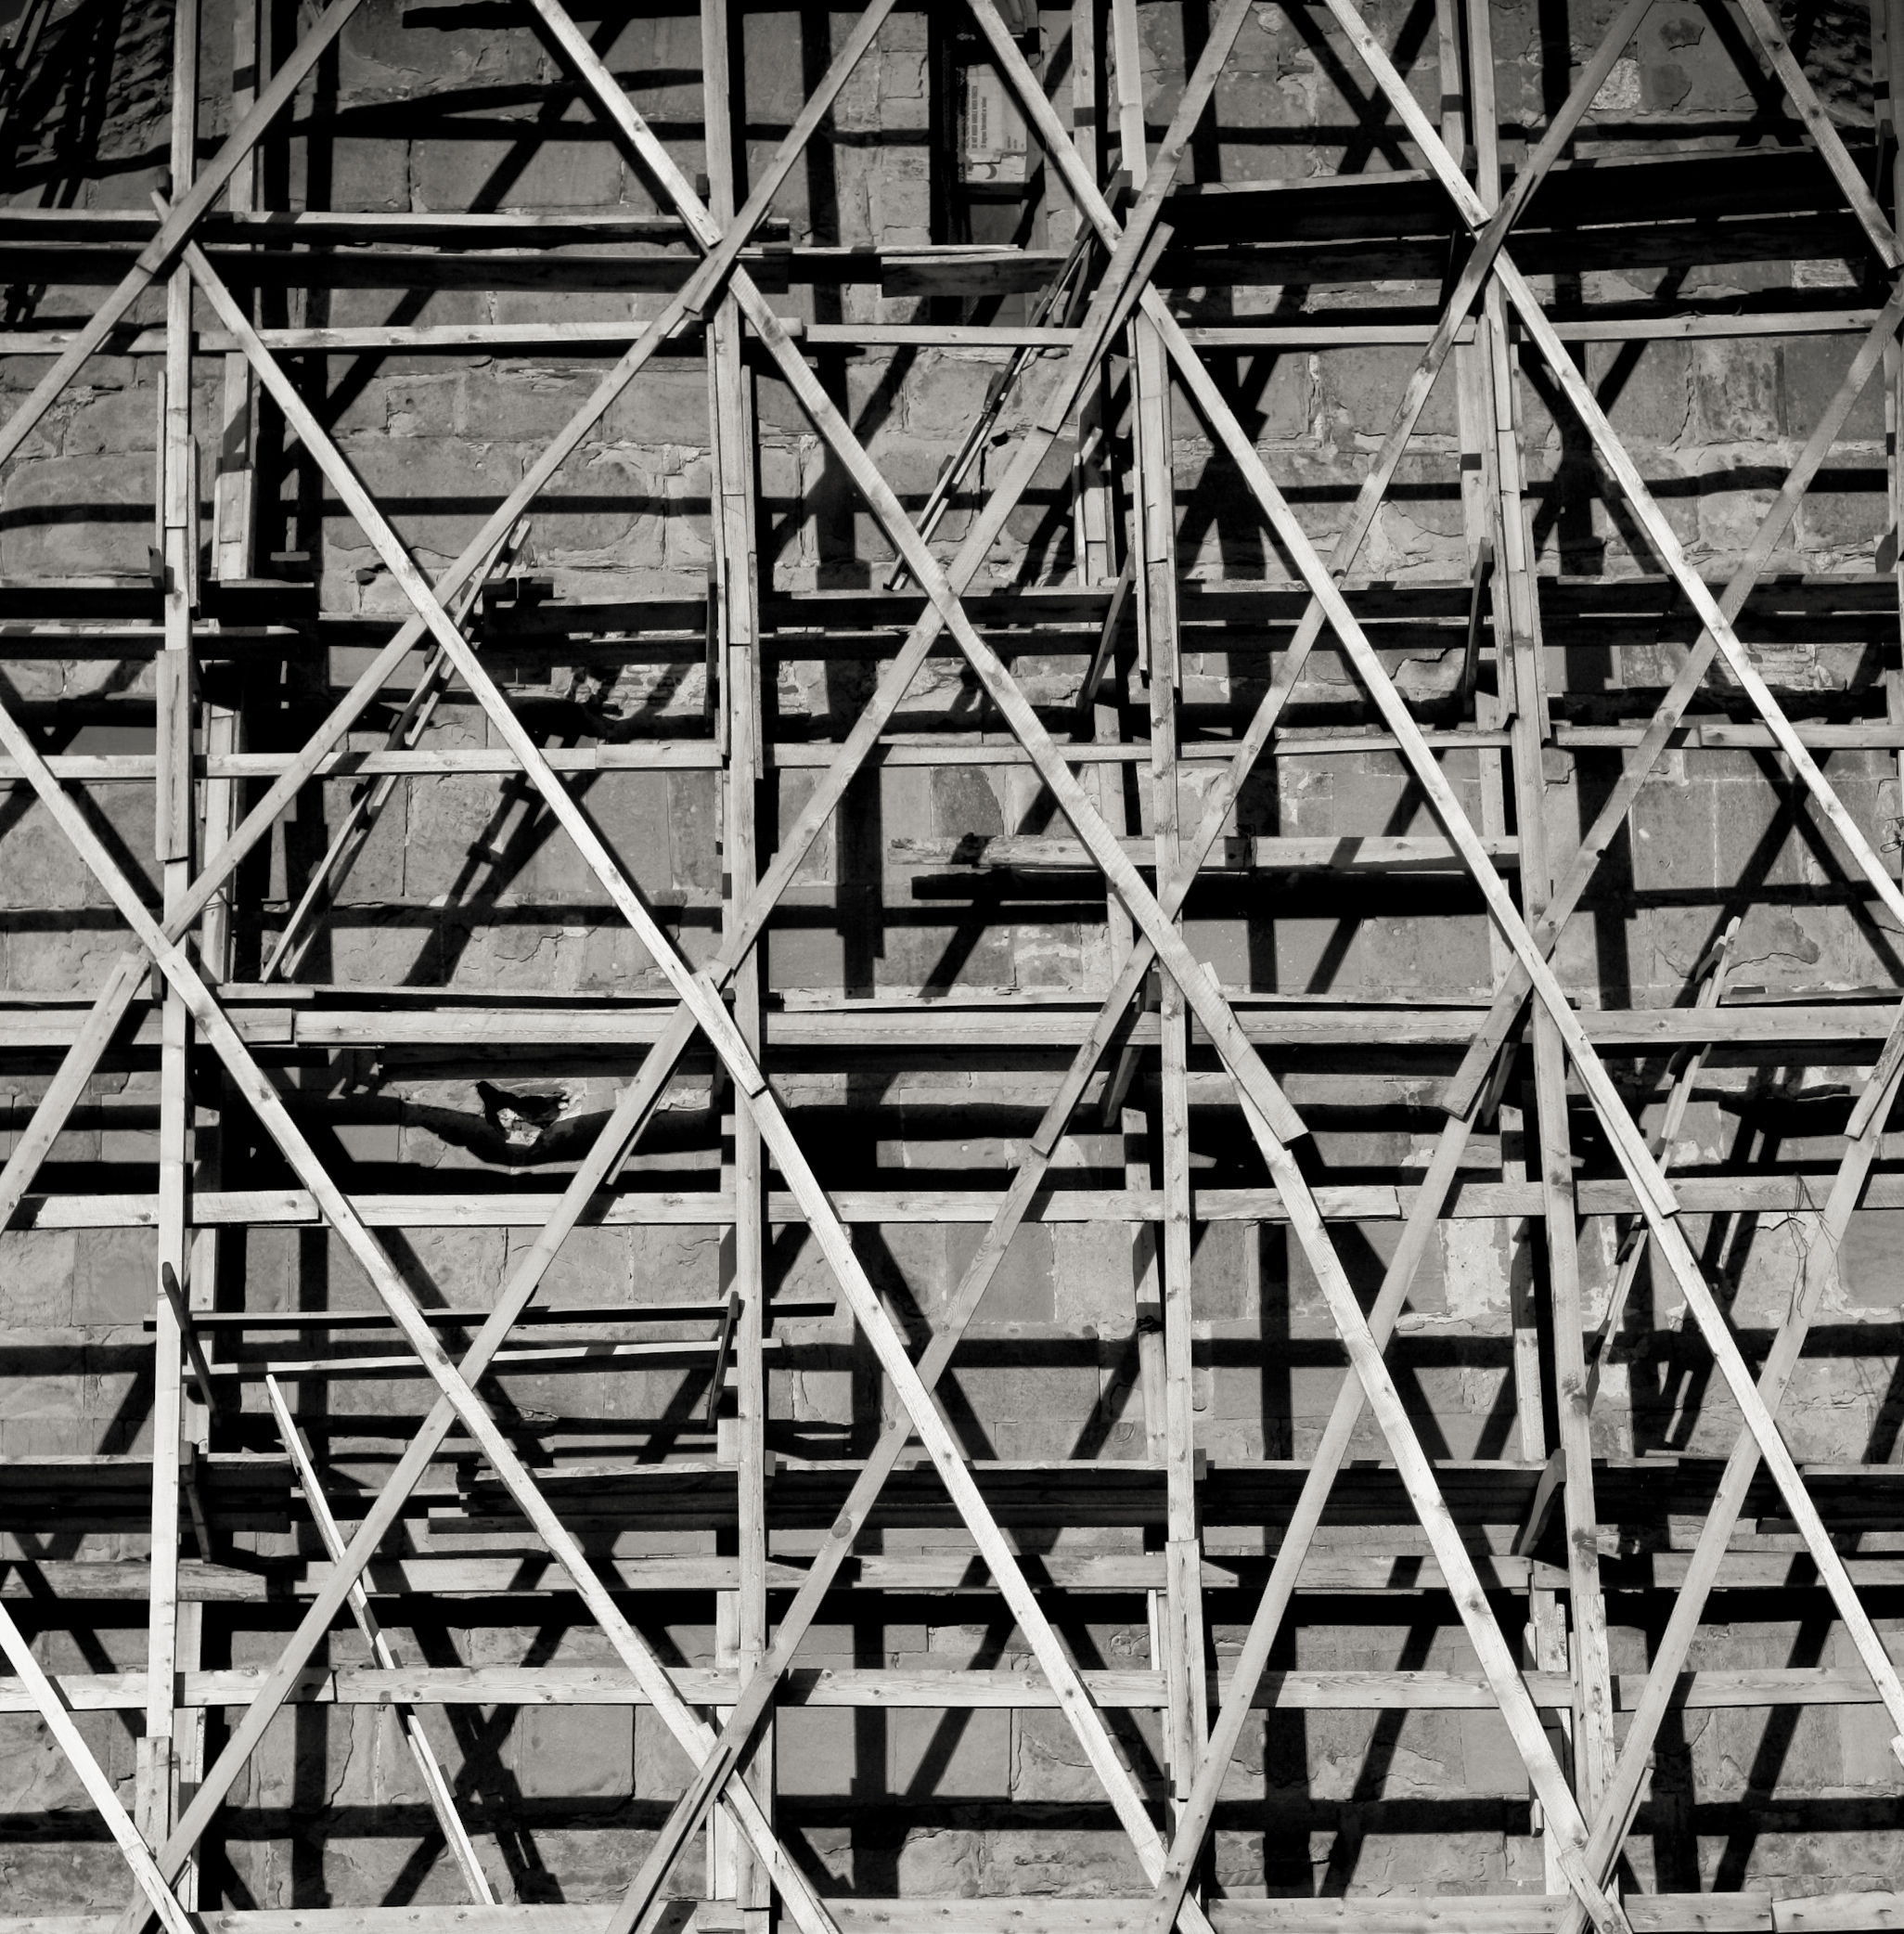
\includegraphics[width=0.95\textwidth]{\folder img/rhombus.jpg}
  \begin{center}
    {\large ``In geometry, a rhombus or rhomb is a quadrilateral 
whose four sides all have the same length''}\par
    Foto di pursanovd\par
    \url{http://www.flickr.com/photos/pursanovd/3669422214/}\par
    Licenza: Creative Commons Attribution 2.0\par
  \end{center}
\newpage

\section{Generalità sui 
quadrilateri}\label{sect:generalita_quadrilateri}

\subsection{Distanza di un punto da una retta e altezza di una 
striscia di piano}

\begin{wrapfigure}{r}{0.3\textwidth}
\centering% Copyright (c) 2015 Daniele Masini - d.masini.it@gmail.com

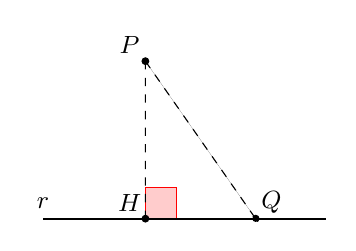
\begin{tikzpicture}[scale=1,font=\small]
\usetikzlibrary{calc}

\begin{scope}
\coordinate (r1) at (0.7,-2);
\coordinate (r2) at (4.3,-2);
\coordinate (s1) at (2,0.5);
\coordinate (s2) at (2,-2.5);
\coordinate (p) at (2,0);
\coordinate (h) at (intersection of r1--r2 and s1--s2);
\coordinate (q) at ($(r1)!0.75!(r2)$);

\draw[red, fill=red!20] (h) rectangle ([shift={(0.4,0.4)}]h);

\draw[thick] (r1) node[above] {$r$} -- (r2);
\draw[dashed] (p) -- (h);
\draw[fill] (p) circle (1.2pt) node [shift={(-.2,.2)}] {$P$};
\draw[fill] (h) circle (1.2pt) node [shift={(-.2,.2)}] {$H$};
\draw[fill,dashed] (p) -- (q) circle (1.2pt) node[shift={(.2,.2)}] {$Q$};

\end{scope}

\end{tikzpicture}

\end{wrapfigure}
Ricordiamo che come definizione di (\emph{misura} della) 
\emph{distanza di un punto da una retta} è stata presa la lunghezza 
del segmento congiungente il punto con il piede della perpendicolare 
mandata dal punto alla retta (vedi figura). Analogamente, per 
\emph{distanza tra due rette parallele}, detta anche \emph{altezza 
della striscia di piano individuata dalle due rette parallele}, si 
intende la distanza di un punto qualsiasi di una retta dall'altra 
retta. Vogliamo far vedere ora che queste definizioni sono coerenti 
con il concetto di distanza tra due insiemi di punti come 
\emph{percorso più breve} che congiunge un qualsiasi punto del primo 
insieme con un generico punto appartenente al secondo insieme. Se 
congiungiamo, infatti, un generico punto \(P\) sia con \(H\), piede della 
perpendicolare alla retta \(r\), che con un altro punto \(Q\in r\), viene 
individuato un triangolo rettangolo \(PHQ\), di cui \(PH\) è un cateto e 
\(PQ\) l'ipotenusa. Dal teorema sulle disuguaglianze degli elementi di 
un triangolo, l'ipotenusa è certamente maggiore di un cateto in 
quanto lato che si oppone ad angolo maggiore (quello retto). Dunque 
\(PH\) è il segmento di lunghezza minore tra tutti quelli che 
congiungono \(P\) con un punto della retta \(r\).

\subsection{Generalità sui poligoni}

Se un poligono ha più di tre lati, allora può anche essere concavo. 
Ricordiamo che la somma degli angoli interni di un quadrilatero è 
\(360\grado\).

\begin{definizione}
Due lati non consecutivi di un quadrilatero si dicono \emph{opposti}; 
analogamente sono detti \emph{opposti} due angoli non adiacenti allo 
stesso lato.
\end{definizione}

Nella figura seguente sono rappresentati un quadrilatero concavo 
(\(Q_1\)), un generico quadrilatero convesso (\(Q_2\)), un quadrilatero 
particolare a forma di ``aquilone'' (\(Q_6\)) e tre quadrilateri 
``notevoli'': \(Q_3\) ha i lati opposti paralleli (a due a due), \(Q_4\) 
e \(Q_5\) hanno una coppia di lati opposti paralleli.


\begin{inaccessibleblock}[Figura: TODO]
 \begin{figure}[htb]
\centering% Copyright (c) 2015 Daniele Masini - d.masini.it@gmail.com

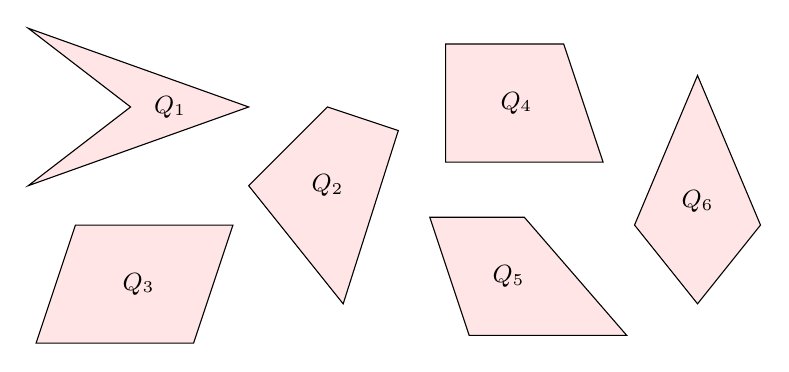
\begin{tikzpicture}[scale=1,font=\small]
\usetikzlibrary{calc}

\begin{scope}
\draw[fill=red!10] (0,0) -- (-1.3,1) -- (1.5,0) -- (-1.3,-1) -- cycle;
\node at (0.5,0) {$Q_1$};
\end{scope}

\begin{scope}[shift={(1.5cm,-1cm)}]
\draw[fill=red!10] (0,0) -- (1,1) -- (1.9,0.7) -- (1.2,-1.5) -- cycle;
\node at (1,0) {$Q_2$};
\end{scope}

\begin{scope}[shift={(-1.2cm,-3cm)}]
\draw[fill=red!10] (0,0) -- (0.5,1.5) -- (2.5,1.5) -- (2,0) -- cycle;
\node at (1.3,0.75) {$Q_3$};
\end{scope}

\begin{scope}[shift={(4cm,-.7cm)}]
\draw[fill=red!10] (0,0) -- (0,1.5) -- (1.5,1.5) -- (2,0) -- cycle;
\node at (0.9,0.75) {$Q_4$};
\end{scope}

\begin{scope}[shift={(4.3cm,-2.9cm)}]
\draw[fill=red!10] (0,0) -- (-0.5,1.5) -- (0.7,1.5) -- (2,0) -- cycle;
\node at (0.5,0.75) {$Q_5$};
\end{scope}

\begin{scope}[shift={(7.2cm,0cm)}]
\draw[fill=red!10] (0,0.4) -- (-0.8,-1.5) -- (0,-2.5) -- (0.8,-1.5) -- cycle;
\node at (0,-1.2) {$Q_6$};
\end{scope}

\end{tikzpicture}

\end{figure}
\end{inaccessibleblock}

I quadrilateri che, come \(Q_6\), hanno due lati consecutivi congruenti 
ed altri due lati consecutivi anch'essi congruenti, si dicono 
\emph{deltoidi}; i quadrilateri che, come \(Q_3\), hanno i lati opposti 
paralleli si dicono \emph{parallelogrammi}; i quadrilateri che, come 
\(Q_4\) e \(Q_5\), hanno una coppia di lati opposti paralleli si dicono 
\emph{trapezi}.

\osservazione In analogia alla definizione di triangolo isoscele 
(come triangolo avente ``almeno'' due lati congruenti), alcuni autori 
definiscono trapezio un quadrilatero avente ``almeno'' una coppia di 
lati opposti paralleli: con questa definizione un parallelogramma è 
un particolare tipo di trapezio. Ricordiamo anche che Euclide, al 
contrario, classificava come trapezi tutti i quadrilateri che non 
fossero parallelogrammi. Noi useremo come definizione di 
\emph{trapezio} quella di un \emph{quadrilatero avente ``solo'' una 
coppia di lati opposti paralleli}. Ci riferiremo al parallelogramma 
come a una figura piana costituita dall'intersezione di due strisce 
di piano non parallele fra loro; al trapezio come intersezione tra 
una striscia di piano ed un angolo convesso con vertice esterno alla 
striscia e lati che intersecano la striscia stessa. Poiché le strisce 
di piano sono convesse, sia i parallelogrammi sia i trapezi, come 
intersezioni di figure convesse, sono convessi.

\section{Trapezio e deltoide}\label{sect:trapezio_deltoide}

Osserviamo le figure seguenti. I quadrilateri \(ABCD\), \(EFGH\), \(IJKL\) 
e \(MNOP\) sono trapezi perché hanno una coppia di lati opposti 
paralleli. Tali lati paralleli si dicono \emph{basi} e si distinguono 
in \emph{base maggiore} e \emph{base minore}. Gli altri lati si 
dicono \emph{lati obliqui}. La distanza tra le rette parallele si 
dice \emph{altezza} del trapezio.
Un trapezio avente i lati obliqui congruenti si dice \emph{isoscele}. 
Un trapezio avente un lato perpendicolare alle basi si dice 
\emph{rettangolo}. Un trapezio che non è né isoscele né rettangolo si 
dice \emph{scaleno}.


\begin{inaccessibleblock}[Figura: TODO]
 \begin{figure}[htb]
	\centering% Copyright (c) 2015 Daniele Masini - d.masini.it@gmail.com

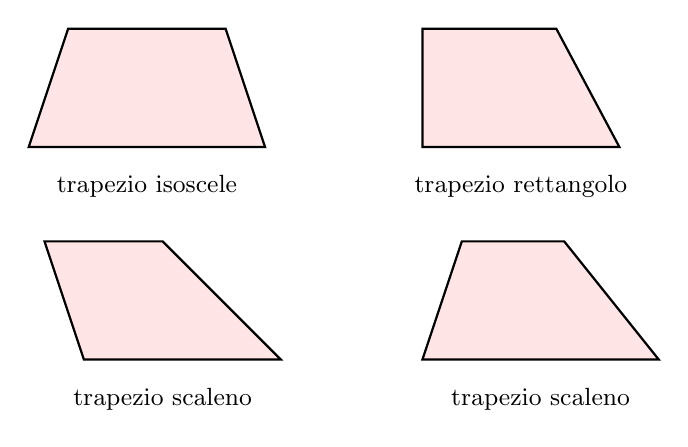
\begin{tikzpicture}[scale=1,font=\small]
\usetikzlibrary{calc}

\begin{scope}
\draw[thick, fill=red!10] (0,0) -- (2,0) -- (2.5,-1.5) -- (-0.5,-1.5) -- cycle;
\node at (1,-2) {trapezio isoscele};
\end{scope}

\begin{scope}[shift={(4.5cm,0cm)}]
\draw[thick, fill=red!10] (0,0) -- (1.7,0) -- (2.5,-1.5) -- (0,-1.5) -- cycle;
\node at (1.25,-2) {trapezio rettangolo};
\end{scope}

\begin{scope}[shift={(-0.3cm,-2.7cm)}]
\draw[thick, fill=red!10] (0,0) -- (1.5,0) -- (3,-1.5) -- (0.5,-1.5) -- cycle;
\node at (1.5,-2) {trapezio scaleno};
\end{scope}

\begin{scope}[shift={(5cm,-2.7cm)}]
\draw[thick, fill=red!10] (0,0) -- (1.3,0) -- (2.5,-1.5) -- (-0.5,-1.5) -- cycle;
\node at (1,-2) {trapezio scaleno};
\end{scope}

\end{tikzpicture}

\end{figure}
\end{inaccessibleblock}

\subsection{Proprietà del trapezio}

In ogni trapezio, gli angoli adiacenti a ciascun lato obliquo sono 
supplementari. Essi, infatti, sono coniugati interni rispetto alle 
rette delle basi tagliate dalla trasversale individuata dal lato 
obliquo.

In un trapezio rettangolo, gli angoli adiacenti alla base maggiore 
sono uno retto ed uno acuto e gli angoli adiacenti alla base minore 
sono uno retto ed uno ottuso. Se un trapezio avesse quattro angoli 
retti, i lati obliqui sarebbero entrambi perpendicolari alle basi e 
di conseguenza paralleli tra loro. Dunque in questo caso il trapezio 
risulterebbe essere un parallelogramma.

Un trapezio scaleno può avere gli angoli adiacenti alla base maggiore 
entrambi acuti (e quindi gli angoli adiacenti alla base minore 
entrambi ottusi) oppure due angoli opposti entrambi acuti e gli altri 
ottusi (i due tipi di trapezio scaleno sono rappresentati nella 
figura precedente). I quattro angoli sono comunque non congruenti, 
altrimenti il trapezio risulterebbe isoscele nel primo caso e un 
parallelogramma nel secondo caso.

\begin{wrapfigure}{r}{0.3\textwidth}
	\centering% Copyright (c) 2015 Daniele Masini - d.masini.it@gmail.com

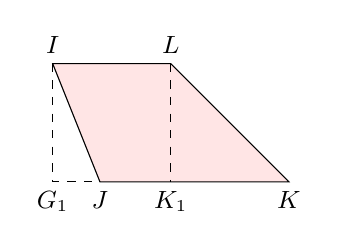
\begin{tikzpicture}[scale=1,font=\small]
\usetikzlibrary{calc}

\begin{scope}
\draw[fill=red!10] (0,0) coordinate (i) node[above] {$I$} -- (1.5,0) coordinate (l) node[above] {$L$} -- (3,-1.5) coordinate (k) node[below] {$K$} -- (0.6,-1.5) coordinate (j) node[below] {$J$} -- cycle;
\draw[dashed] (i) -- ($(j)!(i)!(k)$) coordinate (g1) node[below] {$G_1$} -- (j);
\draw[dashed] (l) -- ($(j)!(l)!(k)$) coordinate (k1) node[below] {$K_1$};
\end{scope}

\end{tikzpicture}

\end{wrapfigure}
In un trapezio isoscele, gli angoli adiacenti alla base maggiore sono 
acuti e quelli adiacenti alla base minore sono ottusi. 
A tal proposito, facciamo riferimento al trapezio \(IJKL\) nella figura 
a fianco per dire che non può esistere un trapezio isoscele con due 
angoli acuti opposti e due angoli ottusi opposti. Infatti, se fosse 
\(IJ\cong LK\), i triangoli \(IG_1J\) e \(LK_1K\) risulterebbero congruenti 
per il criterio particolare dei triangoli rettangoli, avendo 
congruenti le ipotenuse (i lati obliqui del trapezio \(IJ\) e \(LK\)) ed 
una coppia di cateti (le altezze \(IG_1\) e \(LK_1\)), da cui seguirebbe 
in particolare che \(I\widehat{J}G_1\cong L\widehat{K}K_1\), e pertanto 
l'angolo in \(K\) sarebbe supplementare dell'angolo in \(J\), cosa che 
garantirebbe il parallelismo dei lati obliqui. Dunque, un ipotetico 
trapezio isoscele con due angoli acuti opposti sarebbe un 
parallelogramma.

\begin{wrapfigure}{r}{0.3\textwidth}
	\centering% Copyright (c) 2015 Daniele Masini - d.masini.it@gmail.com

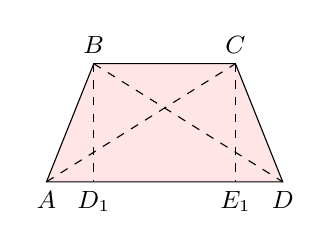
\begin{tikzpicture}[scale=1,font=\small]
\usetikzlibrary{calc}

\begin{scope}
\draw[fill=red!10] (0.1,0) coordinate (b) node[above] {$B$} -- (1.9,0) coordinate (c) node[above] {$C$} -- (2.5,-1.5) coordinate (d) node[below] {$D$} -- (-0.5,-1.5) coordinate (a) node[below] {$A$} -- cycle;
\draw[dashed] (b) -- ($(a)!(b)!(d)$) coordinate (d1) node[below] {$D_1$};
\draw[dashed] (c) -- ($(a)!(c)!(d)$) coordinate (e1) node[below] {$E_1$};
\draw[dashed] (b) -- (d);
\draw[dashed] (a) -- (c);
\end{scope}


\end{tikzpicture}

\end{wrapfigure}
Inoltre, se il trapezio è isoscele, gli angoli adiacenti a ciascuna 
delle basi sono congruenti. 
Infatti, in riferimento al trapezio \(ABCD\), traccia le altezze \(BD_1\) 
e \(CE_1\) (tra loro congruenti perché entrambe rappresentano la 
distanza tra due rette parallele), i triangoli \(AD_1B\) e \(E_1DC\) 
risultano congruenti per il criterio particolare dei triangoli 
rettangoli, avendo congruenti le ipotenuse (i lati obliqui del 
trapezio) ed una coppia di cateti (le altezze del trapezio). Pertanto 
i rimanenti elementi risultano ordinatamente congruenti: 
\(B\widehat{A}D\cong A\widehat{D}C\), \(A\widehat{B}D_1\cong 
D\widehat{C}E_1\), \(AD_1\cong E_1D\).

Dunque sono congruenti  anche le proiezioni dei lati obliqui sulla 
base maggiore. 
Quindi anche \(A\widehat{B}C\cong B\widehat{C}D\) in quanto somme di 
angoli congruenti \(A\widehat{B}D_1+\widehat{R}\cong 
D\widehat{C}E_1+\widehat{R}\).

In un trapezio isoscele, inoltre, anche le due diagonali sono 
congruenti. Infatti, in riferimento sempre al trapezio \(ABCD\) in 
figura, i triangoli \(ABC\) e \(DCB\) risultano congruenti per il primo 
criterio, avendo \(BC\) in comune, \(AB\cong CD\) per ipotesi e gli 
angoli compresi (adiacenti alla base minore) congruenti per quanto 
appena dimostrato. Di conseguenza, i rimanenti elementi sono 
ordinatamente congruenti, in particolare i terzi lati (che sono, 
appunto, le diagonali \(AC\) e \(BD\) del trapezio).

\subsection{Proprietà del deltoide}

\begin{wrapfigure}{r}{0.3\textwidth}
	\centering% Copyright (c) 2015 Daniele Masini - d.masini.it@gmail.com

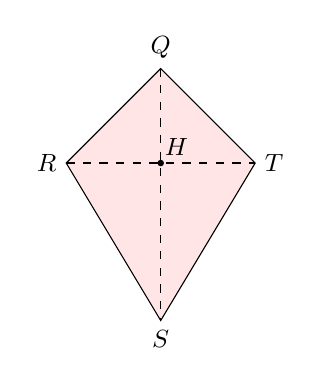
\begin{tikzpicture}[scale=0.8,font=\small]
\usetikzlibrary{calc}

\begin{scope}
\draw[fill=red!10] (0,0) coordinate (q) node[above] {$Q$} -- (1.5,-1.5) coordinate (t) node[right] {$T$} -- (0,-4) coordinate (s) node[below] {$S$} -- (-1.5,-1.5) coordinate (r) node[left] {$R$} -- cycle;
\coordinate (h) at (intersection of r--t and q--s);
\draw[dashed] (q) -- (s);
\draw[dashed] (r) -- (t);
\draw[fill] (h) circle (1.2pt) node[shift={(0.2,0.2)}] {$H$};
\end{scope}


\end{tikzpicture}

\end{wrapfigure}
Il poligono \(QRST\) nella figura a fianco è un deltoide, ha i lati a 
due a due congruenti \(QR\cong QT\) e \(RS\cong TS\). Tracciamo le 
diagonali \(QS\) ed \(RT\). I triangoli \(QRT\) e \(STR\) sono isosceli sulla 
base comune \(RT\). Dunque, se chiamiamo \(H\) il punto medio di \(RT\), 
\(QH\) ed \(SH\) sono mediane, bisettrici e altezze (relative alla base 
ed agli angoli al vertice dei due triangoli isosceli), per cui \(QS\) è 
perpendicolare ad \(RT\) e passa per il punto \(H\). Quindi le due 
diagonali sono perpendicolari e si incontrano nel punto medio di 
\(RT\). Inoltre i triangoli \(SQR\) ed \(STQ\) sono congruenti per il terzo 
criterio, pertanto \(Q\widehat{R}S\cong Q\widehat{T}S\).

I quattro lati di un deltoide non potrebbero essere tutti congruenti, 
in quanto, dalla congruenza degli angoli opposti banalmente 
deducibile, risulterebbero i lati opposti paralleli, e quindi il 
deltoide sarebbe un parallelogramma. Non è al contrario escluso che 
un angolo possa essere retto (ma non più di uno, altrimenti il 
deltoide sarebbe un parallelogramma), mentre gli angoli ottusi possono 
essere uno, due o tre (come pure gli angoli acuti).

Lasciamo al lettore il compito di provare queste semplici proprietà, 
costruendo vari tipi di deltoidi.


\section{Proprietà dei 
parallelogrammi}\label{sect:proprieta_parallelogrammi}

Ricordiamo che, per definizione, un parallelogramma è un quadrilatero 
che ha i lati opposti paralleli.

\begin{teorema}
In ogni parallelogramma:
\begin{enumerate*}
\item gli angoli adiacenti allo stesso lato (a ciascun lato) sono 
supplementari;
\item gli angoli opposti sono congruenti;
\item ciascuna diagonale divide il parallelogramma in due triangoli 
congruenti;
\item i lati opposti sono congruenti;
\item le diagonali si dividono scambievolmente per metà. 
\end{enumerate*}
\end{teorema}

\noindent Ipotesi: \(AB\parallel CD\), \(AD\parallel BC\).


\begin{inaccessibleblock}[Figura: TODO]
 \begin{figure}[htb]
	\centering% Copyright (c) 2015 Daniele Masini - d.masini.it@gmail.com

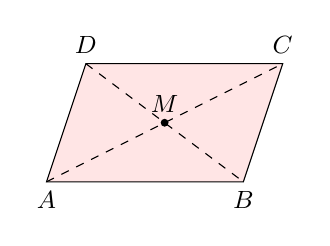
\begin{tikzpicture}[scale=1,font=\small]
\usetikzlibrary{calc}

\begin{scope}
\draw[fill=red!10] (0,0) coordinate (a) node[below] {$A$} -- (2.5,0) coordinate (b) node[below] {$B$} -- (3,1.5) coordinate (c) node[above] {$C$} -- (0.5,1.5) coordinate (d) node[above] {$D$} -- cycle;
\coordinate (m) at (intersection of d--b and a--c);
\draw[dashed] (a) -- (c);
\draw[dashed] (d) -- (b);
\draw[fill] (m) circle (1.2pt) node[above] {$M$};
\end{scope}


\end{tikzpicture}

\end{figure}
\end{inaccessibleblock}

\begin{proof}~\\
\begin{enumerate*}
		
\item Tesi: \(D\widehat{A}B+A\widehat{B}C\cong\pi\), 
\(A\widehat{B}C+B\widehat{C}D\cong\pi\), 
\(B\widehat{C}D+C\widehat{D}A\cong\pi\) (\(\pi\) è l'angolo piatto).\\
Se \(AB\parallel CD\), gli angoli in \(A\) e \(D\) sono supplementari, e 
così pure gli angoli in \(B\) e \(C\), in quanto coniugati interni 
rispetto alle due rette parallele tagliate rispettivamente dalle 
trasversali \(AD\) e \(BC\). Analogamente, se \(AD\parallel BC\), gli 
angoli in \(A\) e \(B\) sono supplementari, ed anche gli angoli in \(C\) e 
\(D\). La tesi 1 è pertanto dimostrata.

\item Tesi: \(A\widehat{B}C\cong C\widehat{D}A\), \(D\widehat{A}B\cong 
B\widehat{C}D\).\\
Dunque, se è vera l'ipotesi, possiamo considerare verificate le 
congruenze della tesi 1. Da queste segue che gli angoli opposti sono 
congruenti in quanto supplementari dello stesso angolo: gli angoli in 
\(A\) e \(C\) sono supplementari entrambi dell'angolo in \(B\), gli angoli 
in \(B\) e in \(D\) sono entrambi supplementari dell'angolo in \(A\). La 
tesi 2 è pertanto dimostrata.

\item Tesi: \(ABC\cong CDA\), \(DAB\cong BCD\).\\
Tracciamo ora una diagonale, ad esempio \(AC\), e consideriamo i due 
triangoli che si vengono a formare, \(ABC\) e \(ACD\). Essendo 
\(AB\parallel CD\), risulta \(D\widehat{C}A\cong C\widehat{A}B\) ed 
essendo \(AD\parallel BC\), risulta \(D\widehat{A}C\cong A\widehat{C}B\), 
in quanto sono coppie di angoli alterni interni, i primi rispetto 
alle rette \(AB\) e \(CD\) tagliate dalla trasversale \(AC\), gli altri 
rispetto alle rette parallele \(AD\) e \(BC\) tagliate dalla trasversale 
\(AC\). I due triangoli dunque, avendo in comune il lato \(AC\), 
risultano congruenti per il secondo criterio. Analogamente, applicando 
il ragionamento precedente ai triangoli \(ABD\) e \(DBC\) dopo aver 
tracciato la diagonale \(DB\), concludiamo che anche i due triangoli 
\(ADB\) e \(DBC\) risultano congruenti per il secondo criterio. Pertanto 
la tesi 3 è dimostrata.

\item Tesi: \(AB\cong CD\), \(AD\cong BC\).\\
Dunque, se è vera l'ipotesi, possiamo considerare verificate le 
congruenze della tesi 3. Dalla congruenza dei triangoli \(ABC\) e \(CDA\) 
segue la congruenza dei lati \(AB\) e \(CD\), dalla congruenza dei 
triangoli \(DAB\) e \(BCD\) segue la congruenza dei lati \(AD\) e \(BC\). 
Pertanto la tesi 4 è dimostrata.

\item Tesi: \(AM\cong MC\), \(DM\cong MB\).\\
Dopo aver tracciato entrambe le diagonali, chiamiamo \(M\) il loro 
punto di intersezione. Confrontiamo i triangoli \(ABM\) e \(CDM\): essi 
risultano congruenti per il secondo criterio, in quanto \(AB\cong CD\) 
(tesi 4), \(D\widehat{A}C\cong A\widehat{C}B\) e \(D\widehat{C}A\cong 
C\widehat{A}B\) (come visto nel punto 3 della dimostrazione). Quindi 
anche i rimanenti elementi risultano ordinatamente congruenti, in 
particolare \(AM\cong MC\) e \(DM\cong MB\). Pertanto anche la tesi 5 è 
dimostrata.
\end{enumerate*}
\end{proof}

Il teorema precedente è invertibile. Precisamente vale il teorema 
seguente:
\begin{teorema}
Se in un quadrilatero è verificata una delle seguenti ipotesi:
\begin{enumerate*}
\item gli angoli adiacenti allo stesso lato (a ciascun lato) sono 
supplementari;
\item gli angoli opposti sono congruenti;
\item ciascuna diagonale divide il quadrilatero in due triangoli 
congruenti;
\item i lati opposti sono congruenti;
\item le diagonali si dividono scambievolmente per metà;
\item due lati opposti sono paralleli e congruenti;
\end{enumerate*}
allora il quadrilatero è un parallelogramma.
\end{teorema}


\begin{inaccessibleblock}[Figura: TODO]
 \begin{figure}[htb]
	\centering% Copyright (c) 2015 Daniele Masini - d.masini.it@gmail.com

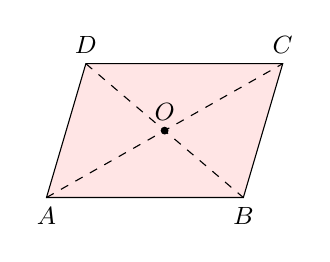
\begin{tikzpicture}[scale=1,font=\small]
\usetikzlibrary{calc}

\begin{scope}
\draw[fill=red!10] (0,0) coordinate (a) node[below] {$A$} -- (2.5,0) coordinate (b) node[below] {$B$} -- (3,1.7) coordinate (c) node[above] {$C$} -- (0.5,1.7) coordinate (d) node[above] {$D$} -- cycle;
\coordinate (o) at (intersection of d--b and a--c);
\draw[dashed] (a) -- (c);
\draw[dashed] (d) -- (b);
\draw[fill] (o) circle (1.2pt) node[above] {$O$};
%\node at (1.5,-1) {(a)};
\end{scope}

%\begin{scope}[xshift=5cm]
%\draw[fill=red!10] (0,0) coordinate (e) node[below] {$E$} -- (2.5,0) coordinate (f) node[below] {$F$} -- (3,1.7) coordinate (g) node[above] {$G$} -- (0.5,1.7) coordinate (h) node[above] {$H$} -- cycle;
%\coordinate (o) at (intersection of d--b and a--c);
%\draw[dashed] (e) -- (g);
%\draw[dashed] (f) -- (h);
%\draw[fill] (o) circle (1.2pt) node[left] {$O$};
%\node at (1.5,-1) {(b)};
%\end{scope}


\end{tikzpicture}

\end{figure}
\end{inaccessibleblock}

\begin{proof}~\\
\begin{enumerate*}
\item Sia per ipotesi \(D\widehat{A}B+A\widehat{B}C\cong \pi\) (dove 
\(\pi\) è l'angolo piatto). Tali angoli, rispetto alle rette \(AD\) ed 
\(BC\) tagliate dalla trasversale \(AB\) sono coniugati interni, allora 
per quanto visto nel capitolo precedente sul parallelismo, le rette 
\(AD\) e \(BC\) sono parallele perché formano angoli coniugati interni 
supplementari con la trasversale \(AB\). Analogamente, se 
\(A\widehat{B}C+B\widehat{C}D\cong \pi\), le rette \(AB\) ed \(DC\) sono 
parallele. Dunque \(ABCD\) è un parallelogramma, avendo i lati opposti 
paralleli.
\item Poiché la somma degli angoli interni di un quadrilatero misura 
\(360\grado\), se gli angoli opposti sono congruenti, vuol dire che 
\(D\widehat{A}B+A\widehat{B}C+B\widehat{C}D+C\widehat{D}A\cong 
2D\widehat{A}B+2A\widehat{B}C\cong 2\pi\), per cui 
\(D\widehat{A}B+A\widehat{B}C\cong\pi\), cioè gli angoli adiacenti allo 
stesso lato sono supplementari e per la dimostrazione precedente 
\(ABCD\) è un parallelogramma.
\item Essendo i triangoli \(ABC\) e \(BDC\) congruenti, l'angolo 
\(A\widehat{B}D\) risulta congruente all'angolo \(B\widehat{D}C\) ed 
essendo questi angoli alterni interni rispetto alle rette \(AB\) e \(CD\) 
tagliate dalla trasversale \(BD\) allora le due rette \(AB\) e \(CD\) 
saranno parallele. In maniera analoga \(A\widehat{D}B\cong 
D\widehat{B}C\) e quindi, essendo alterni interni rispetto alle rette 
\(BC\) e \(AD\) intersecate dalla trasversale \(BD\) si ha che anche 
\(BC\parallel AD\). Quindi \(ABCD\) è un parallelogramma.
%\item Sia \(FH\) una diagonale del quadrilatero \(EFGH\), figura (b), 
allora i vertici \(E\) e \(G\) cadranno su semipiani opposti rispetto 
alla retta \(FH\). Nel caso in cui i due triangoli \(FHE\) e \(FHG\), oltre 
che congruenti, sono isosceli sulla base \(FH\), il quadrilatero \(EFGH\) 
ha gli angoli opposti congruenti, per cui è un parallelogramma per la 
tesi 2. Se, al contrario, \(FHE\) e \(FHG\) non sono isosceli sulla base 
\(FH\), allora dobbiamo considerare due sottocasi distinti, evidenziati 
in figura, con quattro diversi quadrilateri. Se fosse \(EH\cong HG\) e 
\(EF\cong FG\), la figura risulterebbe un deltoide e l'altra diagonale 
\(EG\) non dividerebbe il quadrilatero in due triangoli congruenti. 
Rimane l'altro sottocaso possibile, \(EF\cong HG\) e \(EH\cong FG\), ed 
inoltre \(A\widehat{D}B\cong D\widehat{B}C\), \(A\widehat{B}D\cong 
B\widehat{D}C\) e \(D\widehat{A}B\cong B\widehat{C}D\), pertanto il 
quadrilatero risulta essere un parallelogramma per la 2. Dunque in 
ogni caso possibile la tesi è dimostrata.
\item Consideriamo la diagonale \(AC\). Il quadrilatero \(ABCD\) è diviso 
in due triangoli \(ABC\) e \(ACD\) congruenti per il terzo criterio. 
Pertanto \(A\widehat{C}D\cong C\widehat{A}B\) e \(A\widehat{C}B\cong 
C\widehat{A}D\), coppie di angoli alterni interni, nell'ordine 
rispetto alle rette \(AB\) e \(CD\) e rispetto alle rette \(AD\) ed \(BC\), 
tagliate dalla trasversale \(AC\). Dunque i lati opposti del 
quadrilatero \(ABCD\) risultano paralleli, cioè è un parallelogramma.
\item Detto \(O\) il punto di incontro delle diagonali, i triangoli 
\(OAB\) ed \(OCD\) risultano congruenti per il primo criterio, in quanto 
\(OA\cong OC\), \(OD\cong OB\) e gli angoli tra essi compresi sono 
congruenti perché opposti al vertice. Di conseguenza, risulta anche 
\(D\widehat{C}A\cong C\widehat{A}B\), che sono angoli alterni interni 
rispetto alle rette \(DC\) ed \(AB\) tagliate dalla trasversale \(AC\), 
pertanto \(DC\parallel AB\). Analogamente, considerando i triangoli 
congruenti \(OBC\) ed \(ODA\) si ha anche \(BC\parallel AD\). Dunque \(ABCD\) 
è un parallelogramma.
\item Supponiamo \(AB\) e \(CD\) paralleli e congruenti. Tracciata la 
diagonale \(AC\), risulta \(D\widehat{C}A\cong C\widehat{A}B\) e dunque i 
triangoli \(ACD\) e \(CAB\) risultano congruenti per il primo criterio. 
Di conseguenza risulta \(AD\cong BC\), per cui il quadrilatero ha anche 
l'altra coppia di lati opposti congruenti. \(ABCD\) è dunque un 
parallelogramma per la 4.
\end{enumerate*}
\end{proof}

\section{Parallelogrammi 
particolari}\label{sect:parallelogrammi_particolari}

I parallelogrammi possono essere sia equiangoli sia equilateri.

\noindent\begin{minipage}{0.7\textwidth}\parindent15pt
Se un parallelogramma è equiangolo, dato che la somma degli angoli 
interni è \(360\grado\), deve avere quattro angoli retti: questo 
succede quando due lati opposti, paralleli tra loro, sono 
perpendicolari all’altra coppia di lati opposti. Un tale 
parallelogramma si chiama \emph{rettangolo}.

Se un parallelogramma è equilatero, vuol dire che ciascuna diagonale 
lo divide in due triangoli isosceli. Un tale parallelogramma si 
chiama \emph{rombo}.

Un parallelogramma sia equiangolo sia equilatero deve essere 
contemporaneamente un rettangolo ed un rombo: l'unico tipo di 
quadrilatero regolare, il \emph{quadrato}. Infatti un quadrilatero, 
per essere regolare, deve necessariamente avere quattro angoli retti; 
è quindi un parallelogramma, prima ancora che un rettangolo, perché 
due angoli retti, oltre ad essere congruenti, sono anche 
supplementari; inoltre è un rombo in quanto è un parallelogramma con 
quattro lati congruenti.
\end{minipage}\hfil
\begin{minipage}{0.3\textwidth}
	\centering% Copyright (c) 2015 Daniele Masini - d.masini.it@gmail.com

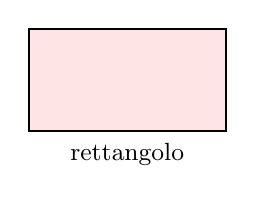
\begin{tikzpicture}[scale=1,font=\small]
\usetikzlibrary{calc}

\begin{scope}
\draw[thick, fill=red!10] (0,0) coordinate (a) -- (2.5,0) coordinate (b) -- (2.5,1.3) coordinate (c) -- (0,1.3) coordinate (d) -- cycle;
\node at (1.25,-0.3) {rettangolo};
\end{scope}

\end{tikzpicture}
\\~\\
	\centering% Copyright (c) 2015 Daniele Masini - d.masini.it@gmail.com

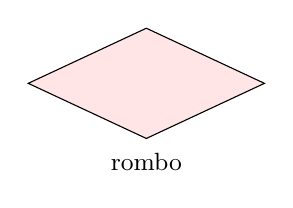
\begin{tikzpicture}[scale=1,font=\small]
\usetikzlibrary{calc}

\begin{scope}
\draw[fill=red!10] (0,0) coordinate (a) -- (1.5,-0.7) coordinate (b) -- (3,0) coordinate (c) -- (1.5,0.7) coordinate (d) -- cycle;
\node at (1.5,-1) {rombo};
\end{scope}

\end{tikzpicture}
\\~\\
	\centering% Copyright (c) 2015 Daniele Masini - d.masini.it@gmail.com

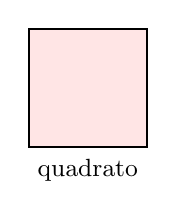
\begin{tikzpicture}[scale=1,font=\small]
\usetikzlibrary{calc}

\begin{scope}
\draw[thick, fill=red!10] (0,0) coordinate (a) -- (1.5,0) coordinate (b) -- (1.5,1.5) coordinate (c) -- (0,1.5) coordinate (d) -- cycle;
\node at (0.75,-0.3) {quadrato};
\end{scope}

\end{tikzpicture}

\end{minipage}

A parte le proprietà particolari insite nelle stesse definizioni, il 
rettangolo e il rombo si distinguono tra loro e dagli altri 
parallelogrammi per alcune proprietà riguardanti le diagonali. 
Naturalmente il quadrato gode delle proprietà sia del rettangolo sia 
del rombo.
Ricordiamo che in un parallelogramma le diagonali si dividono 
scambievolmente per metà. Ora mostreremo che in un rettangolo le 
diagonali sono congruenti ed in un rombo sono perpendicolari.

\begin{teorema}
In ogni rettangolo le diagonali sono congruenti. Viceversa, se un 
parallelogramma ha le diagonali congruenti, allora è un rettangolo.
\end{teorema}


\begin{inaccessibleblock}[Figura: TODO]
 \begin{figure}[htb]
	\centering% Copyright (c) 2015 Daniele Masini - d.masini.it@gmail.com

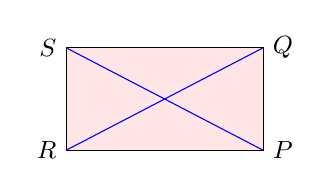
\begin{tikzpicture}[scale=1,font=\small]
\usetikzlibrary{calc}

\begin{scope}
\draw[fill=red!10] (0,0) coordinate (a) node[left] {$R$} -- (2.5,0) coordinate (b) node[right] {$P$} -- (2.5,1.3) coordinate (c) node[right] {$Q$} -- (0,1.3) coordinate (d) node[left] {$S$} -- cycle;
\draw[blue] (a) -- (c);
\draw[blue] (b) -- (d);
\end{scope}

\end{tikzpicture}

\end{figure}
\end{inaccessibleblock}

\begin{proof}
Sia \(RPQS\) un rettangolo; tracciate le diagonali \(RQ\) e \(PS\), 
confrontiamo i triangoli \(SRP\) e \(RPQ\). Tali triangoli rettangoli 
hanno il cateto \(RP\) in comune ed hanno gli altri cateti, \(SR\) e 
\(PQ\), rispettivamente congruenti in quanto lati opposti di un 
rettangolo. Dunque \(SRP\) e \(RPQ\) sono congruenti per il primo criterio 
e di conseguenza devono avere congruenti anche le ipotenuse \(SP\) e 
\(RQ\), le quali sono le diagonali del rettangolo.

Sia \(RPQS\) un parallelogramma avente le diagonali \(RQ\) e \(PS\) 
congruenti, sempre confrontando i triangoli \(SRP\) e \(RPQ\), possiamo 
affermare che tali triangoli sono congruenti per il terzo criterio, 
perché hanno il lato \(RP\) in comune, i lati \(RS\) e \(QP\) congruenti in 
quanto lati opposti di un parallelogramma ed i lati \(SP\) e \(RQ\) 
congruenti per ipotesi. Dunque anche gli angoli devono essere 
ordinatamente congruenti, in particolare  perché opposti ai lati 
congruenti \(SP\) e \(RQ\). Ma tali angoli sono anche supplementari in 
quanto adiacenti allo stesso lato \(RP\) di un parallelogramma e 
pertanto devono risultare retti. Dunque il quadrilatero \(RPSQ\) è un 
rettangolo.
\end{proof}

\begin{teorema}
In ogni rombo le diagonali sono perpendicolari e sono anche 
bisettrici degli angoli aventi per vertici i loro estremi. Viceversa, 
se un parallelogramma ha le diagonali perpendicolari è un rombo; 
inoltre, se un angolo di un parallelogramma è diviso a metà dalla 
diagonale passante per il suo vertice, allora il parallelogramma è un 
rombo.
\end{teorema}


\begin{inaccessibleblock}[Figura: TODO]
 \begin{figure}[htb]
	\centering% Copyright (c) 2015 Daniele Masini - d.masini.it@gmail.com

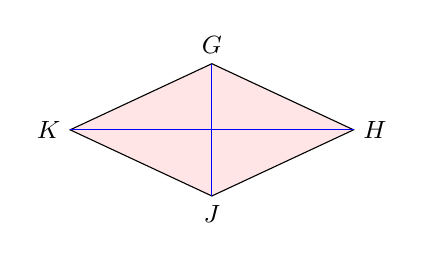
\begin{tikzpicture}[scale=1.2,font=\small]
\usetikzlibrary{calc}

\begin{scope}
\draw[fill=red!10] (0,0) coordinate (a) node[left] {$K$} -- (1.5,-0.7) coordinate (b) node[below] {$J$} -- (3,0) coordinate (c) node[right] {$H$} -- (1.5,0.7) coordinate (d) node[above] {$G$} -- cycle;
\draw[blue] (a) -- (c);
\draw[blue] (b) -- (d);
\end{scope}

\end{tikzpicture}

\end{figure}
\end{inaccessibleblock}

\begin{proof}
Notiamo che, in ciascuna delle fasi della dimostrazione, è tra le 
ipotesi del teorema che \(JHGK\) sia un parallelogramma. Ricordiamo che 
le diagonali di \(JHGK\) vengono divise a metà dal loro punto di 
intersezione, che chiamiamo \(M\), per cui risulta \(JM\cong MG\) e 
\(HM\cong MK\).
\begin{enumeratea}
\item Se supponiamo che \(JHGK\) sia un rombo, i triangoli \(JHG\), 
\(HGK\), \(GKJ\) e \(KJH\) risultano isosceli, per cui le mediane \(HM\), 
\(GM\), \(KM\) e \(JM\) sono anche altezze e bisettrici, per cui la prima 
parte del teorema è dimostrata.
\item Se supponiamo che \(JG\) e \(HK\) siano perpendicolari, in 
particolare i triangoli rettangoli \(JHM\), \(HGM\), \(GKM\) e \(KJM\) 
risultano congruenti per il primo criterio, avendo congruenti i 
cateti. Dunque risultano congruenti anche le ipotenuse, che sono i 
lati del parallelogramma \(JHGK\), il quale pertanto risulta essere un 
rombo.
\item Se supponiamo ad esempio \(K\widehat{G}J\cong J\widehat{G}H\), 
essendo anche \(K\widehat{G}J\cong G\widehat{J}H\) in quanto alterni 
interni rispetto alle rette parallele \(KG\) e \(JH\) tagliate dalla 
trasversale \(GJ\), dalla proprietà transitiva della congruenza segue 
che \(G\widehat{J}H\cong J\widehat{G}H\), per cui il triangolo \(JGH\) 
risulta isoscele sulla base \(JG\). Dunque il parallelogramma \(JHGK\) ha 
due lati consecutivi congruenti, e quindi i quattro lati congruenti, 
ed è pertanto un rombo.
\end{enumeratea}
\end{proof}

I teoremi precedenti si estendono automaticamente ai quadrati.
\begin{corollario}
Le diagonali di un quadrato sono fra loro congruenti e perpendicolari 
e dividono per metà gli angoli. Viceversa, se un parallelogramma ha 
le diagonali congruenti e perpendicolari, allora è un quadrato; 
inoltre, se le diagonali di un parallelogramma sono congruenti ed un 
angolo è diviso a metà da una diagonale, allora il parallelogramma è 
un quadrato.
\end{corollario}

\section{Corrispondenza di Talete}\label{sect:corrispondenza_talete}

\begin{definizione}
Nel piano, si definisce \emph{fascio improprio di rette} un insieme 
di rette tutte parallele tra loro.
\end{definizione}

Ricordiamo che una retta contenuta nello stesso piano e non 
appartenente al fascio improprio è necessariamente incidente rispetto 
a ciascuna retta del fascio ed ha quindi uno ed un solo punto in 
comune con ogni singola retta del fascio: una tale retta è dunque una 
trasversale.

\noindent\begin{minipage}{0.65\textwidth}\parindent15pt
Dato un fascio di rette parallele \(a\), \(b\), \(c\), \(d\), \ldots{}, 
considerate due generiche trasversali, \(t_1\) e \(t_2\), è possibile 
definire una funzione tra l'insieme dei punti di una trasversale e 
quello dei punti dell'altra trasversale, che associ a ciascun punto 
di \(t_1\) il punto di \(t_2\) che appartiene alla medesima retta del 
fascio (ad esempio al punto \(A_1\) si associa il punto \(A_2\) se, come 
nella figura a fianco, \(A_1 = a \cap t_1\) e \(A_2 = a \cap t_2\)). Tale 
funzione è una corrispondenza biunivoca e si estende facilmente ai 
segmenti: infatti l'immagine del segmento \(A_1B_1\) è il segmento 
\(A_2B_2\) (se, come nella figura, anche gli estremi \(B_1\) e \(B_2\) 
appartengono alla stessa retta \(b\) del fascio).
La corrispondenza biunivoca così definita tra punti e tra segmenti di 
due trasversali che tagliano un fascio di rette parallele è nota come 
\emph{corrispondenza di Talete}.
\end{minipage}\hfil
\begin{minipage}{0.35\textwidth}
	\centering% Copyright (c) 2015 Daniele Masini - d.masini.it@gmail.com

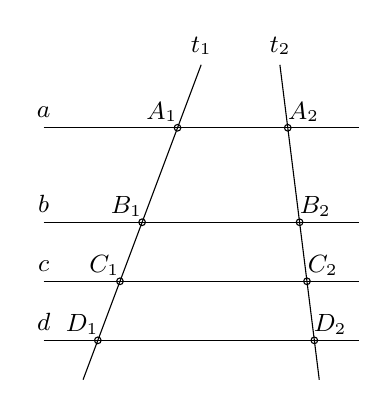
\begin{tikzpicture}[scale=1,font=\small]
\usetikzlibrary{calc}

\begin{scope}
\coordinate (a1) at (0,-0.3);
\coordinate (a2) at (4,-0.3);
\coordinate (b1) at (0,-1.5);
\coordinate (b2) at (4,-1.5);
\coordinate (c1) at (0,-2.25);
\coordinate (c2) at (4,-2.25);
\coordinate (d1) at (0,-3);
\coordinate (d2) at (4,-3);
\coordinate (t11) at (2,0.5);
\coordinate (t12) at (0.5,-3.5);
\coordinate (t21) at (3,0.5);
\coordinate (t22) at (3.5,-3.5);
\coordinate (A1) at (intersection of a1--a2 and t11--t12);
\coordinate (A2) at (intersection of a1--a2 and t21--t22);
\coordinate (B1) at (intersection of b1--b2 and t11--t12);
\coordinate (B2) at (intersection of b1--b2 and t21--t22);
\coordinate (C1) at (intersection of c1--c2 and t11--t12);
\coordinate (C2) at (intersection of c1--c2 and t21--t22);
\coordinate (D1) at (intersection of d1--d2 and t11--t12);
\coordinate (D2) at (intersection of d1--d2 and t21--t22);

\draw (a1) node[above] {$a$} -- (a2);
\draw (b1) node[above] {$b$} -- (b2);
\draw (c1) node[above] {$c$} -- (c2);
\draw (d1) node[above] {$d$} -- (d2);
\draw (t11) node[above] {$t_1$} -- (t12);
\draw (t21) node[above] {$t_2$} -- (t22);
\draw (A1) circle (1.2pt) node[shift={(-0.2,0.2)}] {$A_1$};
\draw (A2) circle (1.2pt) node[shift={(0.2,0.2)}] {$A_2$};
\draw (B1) circle (1.2pt) node[shift={(-0.2,0.2)}] {$B_1$};
\draw (B2) circle (1.2pt) node[shift={(0.2,0.2)}] {$B_2$};
\draw (C1) circle (1.2pt) node[shift={(-0.2,0.2)}] {$C_1$};
\draw (C2) circle (1.2pt) node[shift={(0.2,0.2)}] {$C_2$};
\draw (D1) circle (1.2pt) node[shift={(-0.2,0.2)}] {$D_1$};
\draw (D2) circle (1.2pt) node[shift={(0.2,0.2)}] {$D_2$};

\end{scope}

\end{tikzpicture}

\end{minipage}

\begin{teorema}
Dato un fascio di rette parallele tagliato da due trasversali, a 
segmenti congruenti su una trasversale corrispondono segmenti 
congruenti sull'altra trasversale.
\end{teorema}

\noindent Ipotesi: \(A\parallel b\parallel c\parallel d\), \(t_1\) e 
\(t_2\) trasversali, \(A_1B_1\cong C_1D_1\).\tab Tesi: \(A_2B_2\cong 
C_2D_2\).


\begin{inaccessibleblock}[Figura: TODO]
 \begin{figure}[htb]
	\centering% Copyright (c) 2015 Daniele Masini - d.masini.it@gmail.com

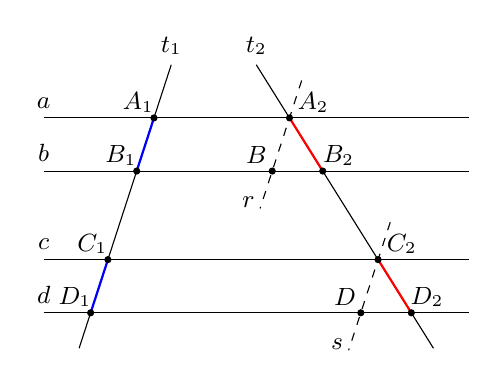
\begin{tikzpicture}[scale=0.9,font=\small, extended line/.style={shorten >=-#1,shorten <=-#1},
  extended line/.default=0.5cm]
\usetikzlibrary{calc}

\begin{scope}
\coordinate (a1) at (0,-.25);
\coordinate (a2) at (6,-.25);
\coordinate (b1) at (0,-1);
\coordinate (b2) at (6,-1);
\coordinate (c1) at (0,-2.25);
\coordinate (c2) at (6,-2.25);
\coordinate (d1) at (0,-3);
\coordinate (d2) at (6,-3);
\coordinate (t11) at (1.8,0.5);
\coordinate (t12) at (0.5,-3.5);
\coordinate (t21) at (3,0.5);
\coordinate (t22) at (5.5,-3.5);
\coordinate (A1) at (intersection of a1--a2 and t11--t12);
\coordinate (A2) at (intersection of a1--a2 and t21--t22);
\coordinate (B1) at (intersection of b1--b2 and t11--t12);
\coordinate (B2) at (intersection of b1--b2 and t21--t22);
\coordinate (C1) at (intersection of c1--c2 and t11--t12);
\coordinate (C2) at (intersection of c1--c2 and t21--t22);
\coordinate (D1) at (intersection of d1--d2 and t11--t12);
\coordinate (D2) at (intersection of d1--d2 and t21--t22);
\path (A2) -- +($(B1)-(A1)$) coordinate (B);
\path (C2) -- +($(D1)-(C1)$) coordinate (D);
\draw[dashed, extended line] (A2) -- (B) node[shift={(-.3,-.4)}] {$r$};
\draw[dashed, extended line] (C2) -- (D) node[shift={(-.3,-.4)}] {$s$};

\draw (a1) node[above] {$a$} -- (a2);
\draw (b1) node[above] {$b$} -- (b2);
\draw (c1) node[above] {$c$} -- (c2);
\draw (d1) node[above] {$d$} -- (d2);
\draw (t11) node[above] {$t_1$} -- (t12);
\draw (t21) node[above] {$t_2$} -- (t22);
\draw[thick, blue] (A1) -- (B1);
\draw[thick, blue] (C1) -- (D1);
\draw[thick, red] (A2) -- (B2);
\draw[thick, red] (C2) -- (D2);
\draw[fill] (A1) circle (1.2pt) node[shift={(-0.2,0.2)}] {$A_1$};
\draw[fill] (A2) circle (1.2pt) node[shift={(0.3,0.2)}] {$A_2$};
\draw[fill] (B1) circle (1.2pt) node[shift={(-0.2,0.2)}] {$B_1$};
\draw[fill] (B2) circle (1.2pt) node[shift={(0.2,0.2)}] {$B_2$};
\draw[fill] (C1) circle (1.2pt) node[shift={(-0.2,0.2)}] {$C_1$};
\draw[fill] (C2) circle (1.2pt) node[shift={(0.3,0.2)}] {$C_2$};
\draw[fill] (D1) circle (1.2pt) node[shift={(-0.2,0.2)}] {$D_1$};
\draw[fill] (D2) circle (1.2pt) node[shift={(0.2,0.2)}] {$D_2$};
\draw[fill] (B) circle (1.2pt) node[shift={(-0.2,0.2)}] {$B$};
\draw[fill] (D) circle (1.2pt) node[shift={(-0.2,0.2)}] {$D$};

\end{scope}

\end{tikzpicture}

\end{figure}
\end{inaccessibleblock}

\begin{proof}
Se fosse \(t_1\parallel t_2\), allora la tesi seguirebbe facilmente 
dalle proprietà dei quadrilateri particolari e dalla proprietà 
transitiva della congruenza. Infatti i quadrilateri \(A_1B_1B_2A_2\) e 
\(C_1D_1D_2C_2\) sarebbero due parallelogrammi, ed avrebbero dunque i 
lati opposti congruenti.
Altrimenti, tracciamo la retta \(r\) passante per \(A_2\) e la retta \(s\) 
passante per \(C_2\), entrambe parallele a \(t_1\); chiamiamo \(B\) il 
punto di intersezione tra \(b\) ed \(r\) e \(D\) il punto di intersezione 
tra \(d\) ed \(s\).
I quadrilateri \(A_1B_1BA_2\) e \(C_1D_1DC_2\) sono due parallelogrammi, 
per cui da \(A_1B_1\cong C_1D_1\) segue, per la proprietà transitiva 
della congruenza, \(A_2B\cong C_2D\). Dunque, se confrontiamo i 
triangoli \(A_2BB_2\) e \(C_2DD_2\), questi risultano congruenti per il 
secondo criterio (generalizzato), in quanto gli angoli in \(A_2\) e in 
\(C_2\) sono corrispondenti rispetto alle rette parallele \(r\) e \(s\) 
tagliate dalla trasversale \(t_2\), mentre gli angoli in \(B_2\) e \(D_2\) 
sono corrispondenti rispetto alle rette parallele \(b\) e \(d\) tagliate 
dalla trasversale \(t_2\) e pertanto congruenti. Di conseguenza 
\(A_2B_2\cong C_2D_2\).
\end{proof}

\noindent\begin{minipage}{0.6\textwidth}\parindent15pt
\osservazione Nella figura precedente, i trapezi \(A_1B_1B_2A_2\) e 
\(C_1D_1D_2C_2\) sono stati ``decomposti'' in parallelogrammi e 
triangoli. La sostanza del teorema non cambia però se le figure che 
si ottengono sono diverse.
Nella figura seguente, si considerino, oltre alla corrispondenza tra 
i segmenti su \(t_1\) e \(t_2\), anche le corrispondenze tra i segmenti 
su \(t_1\) e \(t_3\) (parallele) e quella tra i segmenti su \(t_2\) e \(t_3\) 
(con \(C_3\) coincidente con \(C_2\)).
\end{minipage}\hfil
\begin{minipage}{0.4\textwidth}
	\centering% Copyright (c) 2015 Daniele Masini - d.masini.it@gmail.com

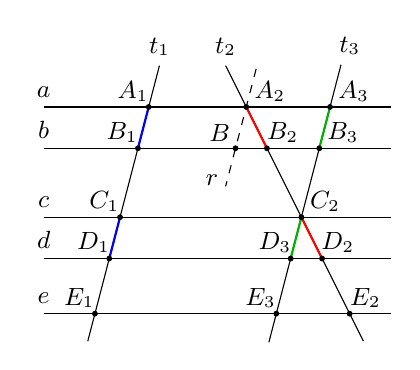
\begin{tikzpicture}[scale=.7,font=\small, extended line/.style={shorten >=-#1,shorten <=-#1},
  extended line/.default=0.5cm]
\usetikzlibrary{calc}

\begin{scope}
\coordinate (a1) at (-0.3,-.25);
\coordinate (a2) at (6,-.25);
\coordinate (b1) at (-0.3,-1);
\coordinate (b2) at (6,-1);
\coordinate (c1) at (-0.3,-2.25);
\coordinate (c2) at (6,-2.25);
\coordinate (d1) at (-0.3,-3);
\coordinate (d2) at (6,-3);
\coordinate (e1) at (-0.3,-4);
\coordinate (e2) at (6,-4);
\coordinate (t11) at (1.8,0.5);
\coordinate (t12) at (0.5,-4.5);
\coordinate (t21) at (3,0.5);
\coordinate (t22) at (5.5,-4.5);
\coordinate (A1) at (intersection of a1--a2 and t11--t12);
\coordinate (A2) at (intersection of a1--a2 and t21--t22);
\coordinate (B1) at (intersection of b1--b2 and t11--t12);
\coordinate (B2) at (intersection of b1--b2 and t21--t22);
\coordinate (C1) at (intersection of c1--c2 and t11--t12);
\coordinate (C2) at (intersection of c1--c2 and t21--t22);
\coordinate (D1) at (intersection of d1--d2 and t11--t12);
\coordinate (D2) at (intersection of d1--d2 and t21--t22);
\coordinate (E1) at (intersection of e1--e2 and t11--t12);
\coordinate (E2) at (intersection of e1--e2 and t21--t22);
\path (A2) -- +($(B1)-(A1)$) coordinate (B);
\path (C2) -- +($(D1)-(C1)$) coordinate (D);
\draw[dashed, extended line] (A2) -- (B) node[shift={(-.3,-.4)}] {$r$};
\draw[shorten >=-1.1cm,shorten <=-2cm] (C2) -- (D) node[shift={(.75,2.7)}] {$t_3$};
\coordinate (A3) at (intersection of a1--a2 and C2--D);
\coordinate (B3) at (intersection of b1--b2 and C2--D);
\coordinate (E3) at (intersection of e1--e2 and C2--D);


\draw (a1) node[above] {$a$} -- (a2);
\draw (b1) node[above] {$b$} -- (b2);
\draw (c1) node[above] {$c$} -- (c2);
\draw (d1) node[above] {$d$} -- (d2);
\draw (e1) node[above] {$e$} -- (e2);
\draw (t11) node[above] {$t_1$} -- (t12);
\draw (t21) node[above] {$t_2$} -- (t22);
\draw[thick, blue] (A1) -- (B1);
\draw[thick, blue] (C1) -- (D1);
\draw[thick, red] (A2) -- (B2);
\draw[thick, red] (C2) -- (D2);
\draw[thick, green!70!black] (A3) -- (B3);
\draw[thick, green!70!black] (C2) -- (D);
\draw[fill] (A1) circle (1.2pt) node[shift={(-0.2,0.2)}] {$A_1$};
\draw[fill] (A2) circle (1.2pt) node[shift={(0.3,0.2)}] {$A_2$};
\draw[fill] (A3) circle (1.2pt) node[shift={(0.3,0.2)}] {$A_3$};
\draw[fill] (B1) circle (1.2pt) node[shift={(-0.2,0.2)}] {$B_1$};
\draw[fill] (B2) circle (1.2pt) node[shift={(0.2,0.2)}] {$B_2$};
\draw[fill] (B3) circle (1.2pt) node[shift={(0.3,0.2)}] {$B_3$};
\draw[fill] (C1) circle (1.2pt) node[shift={(-0.2,0.2)}] {$C_1$};
\draw[fill] (C2) circle (1.2pt) node[shift={(0.3,0.2)}] {$C_2$};
\draw[fill] (D1) circle (1.2pt) node[shift={(-0.2,0.2)}] {$D_1$};
\draw[fill] (D2) circle (1.2pt) node[shift={(0.2,0.2)}] {$D_2$};
\draw[fill] (E1) circle (1.2pt) node[shift={(-0.2,0.2)}] {$E_1$};
\draw[fill] (E2) circle (1.2pt) node[shift={(0.2,0.2)}] {$E_2$};
\draw[fill] (E3) circle (1.2pt) node[shift={(-0.2,0.2)}] {$E_3$};
\draw[fill] (B) circle (1.2pt) node[shift={(-0.2,0.2)}] {$B$};
\draw[fill] (D) circle (1.2pt) node[shift={(-0.2,0.2)}] {$D_3$};

\end{scope}

\end{tikzpicture}

\end{minipage}


\section{Conseguenze della corrispondenza di 
Talete}\label{sect:conseguenze_corrispondenza_talete}

\begin{corollario}
Se dal punto medio di un lato di un triangolo tracciamo la parallela 
ad un altro lato del triangolo, questa interseca il terzo lato nel 
suo punto medio.
\end{corollario}

\noindent\begin{minipage}{0.65\textwidth}\parindent15pt
\begin{proof}
Sia \(M\) il punto medio di \(AC\), sia \(r\) la parallela ad \(AB\) passante 
per \(M\), sia \(N\) il punto di intersezione tra \(r\) e \(CB\),  sia \(s\) la 
parallela ad \(AB\) passante per \(C\). Poiché per ipotesi \(CM\cong MA\), 
per la corrispondenza di Talete risulta \(CN\cong NB\), per cui \(N\) è 
il punto medio di \(CB\).
\end{proof}
\end{minipage}\hfil
\begin{minipage}{0.35\textwidth}
	\centering% Copyright (c) 2015 Daniele Masini - d.masini.it@gmail.com

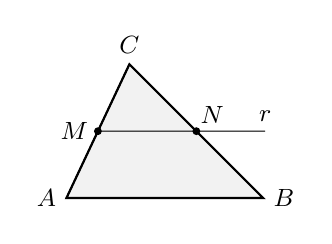
\begin{tikzpicture}[scale=1,font=\small]
\usetikzlibrary{calc, through, intersections}

\begin{scope}
\coordinate (a) at (0,0);
\coordinate (b) at (0.8,1.7);
\coordinate (c) at (2.5,0);
\draw[fill=gray!10] (a) -- (b) -- (c) -- cycle;

\coordinate (m) at ($(a)!.5!(b)$);

\path (m) -- +($(c)-(a)$) coordinate (r2);

\draw[fill] (m) circle (1.2pt) node[left] {$M$} -- ($(m)!0.85!(r2)$) node[above] {$r$};
\coordinate (n) at (intersection of m--r2 and b--c);
\draw[fill] (n) circle (1.2pt) node[shift={(0.2,0.2)}] {$N$};

\draw[thick] (a) node[left] {$A$} -- (b) node[above] {$C$} -- (c) node[right] {$B$} -- cycle;

\end{scope}

\end{tikzpicture}

\end{minipage}

\begin{corollario}
Il segmento congiungente i punti medi di due lati di un triangolo è 
parallelo al terzo lato e congruente alla sua metà.
\end{corollario}

\noindent\begin{minipage}{0.65\textwidth}\parindent15pt
\begin{proof}
Sia \(M\) il punto medio di \(AC\) e sia \(N\) il punto medio di \(CB\). 
Poiché, per il corollario precedente, la parallela ad \(AB\) passante 
per \(M\) passa anche per \(N\), il segmento \(MN\) è parallelo ad \(AB\) (in 
quanto una retta è ben individuata da due punti ed inoltre, per il 
quinto postulato di Euclide, esiste una ed una sola retta passante 
per \(M\) e parallela ad \(AB\)). Rimane da dimostrare che \(MN\cong 
\frac{1}{2}AB\). Sempre per il corollario precedente, se da \(M\) 
tracciamo la parallela a \(CB\), questa interseca \(AB\) nel suo punto 
medio \(K\). Il quadrilatero \(MKBN\) è un parallelogramma, in quanto ha 
i lati opposti paralleli. Per le proprietà dei parallelogrammi, 
\(MN\cong KB\cong \frac{1}{2}AB\).
\end{proof}
\end{minipage}\hfil
\begin{minipage}{0.35\textwidth}
	\centering% Copyright (c) 2015 Daniele Masini - d.masini.it@gmail.com

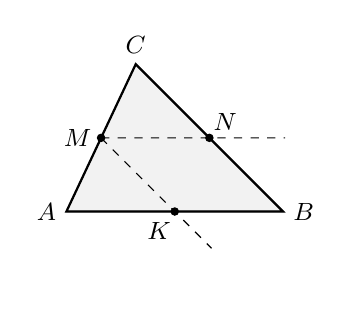
\begin{tikzpicture}[scale=1.1,font=\small]
\usetikzlibrary{calc, through, intersections}

\begin{scope}
\coordinate (a) at (0,0);
\coordinate (b) at (0.8,1.7);
\coordinate (c) at (2.5,0);
\draw[fill=gray!10] (a) -- (b) -- (c) -- cycle;

\coordinate (m) at ($(a)!.5!(b)$);

\path (m) -- +($(c)-(a)$) coordinate (r2);
\path (m) -- +($(c)-(b)$) coordinate (s2);

\draw[fill] (m) circle (1.2pt) node[left] {$M$};
\draw[dashed] (m) -- ($(m)!0.85!(r2)$);
\coordinate (n) at (intersection of m--r2 and b--c);
\draw[fill] (n) circle (1.2pt) node[shift={(0.2,0.2)}] {$N$};
\draw[dashed] (m) -- ($(m)!0.75!(s2)$);
\coordinate (k) at (intersection of m--s2 and a--c);
\draw[fill] (k) circle (1.2pt) node[shift={(-0.2,-0.25)}] {$K$};

\draw[thick] (a) node[left] {$A$} -- (b) node[above] {$C$} -- (c) node[right] {$B$} -- cycle;

\end{scope}

\end{tikzpicture}

\end{minipage}

% \newpage
% 
% \input{./chap/04_esercizi}
% 
% \cleardoublepage
